\documentclass[preprint,12pt]{elsarticle}

\usepackage{amsmath,amssymb}
\usepackage{booktabs}
\usepackage{graphicx}
\usepackage{multirow}
\usepackage{siunitx}
\usepackage{url}
\usepackage{xcolor}
\usepackage{microtype}
\usepackage{enumitem}
\usepackage{threeparttable}
\usepackage[hidelinks]{hyperref}

\journal{Machine Learning with Applications}
\emergencystretch=2em
\biboptions{sort&compress}

\begin{document}

\begin{frontmatter}

\title{AudioTwin: Safety-Constrained Preferential Bayesian Optimisation for Query-Efficient Personalised Hearing-Aid Fitting}

\author[uow]{Alan Immanuel Benjamin Vallavaraj}
\ead{a.vallavaraj@westminster.ac.uk}
\address[uow]{School of Computer Science and Engineering, University of Westminster, London, United Kingdom}

\begin{abstract}
Personalisation problems often require optimisation of an unknown subjective utility function from a small number of user interactions while respecting hard operational constraints. We present \textit{AudioTwin}, a safety-constrained preferential Bayesian optimisation framework evaluated for personalised hearing-aid fitting. AudioTwin represents candidate processing configurations in a six-dimensional latent space controlling gain, spectral tilt, compression, noise reduction, speech enhancement and compression speed. Listener-specific utility is learned from noisy pairwise preferences using a Gaussian-process preference model with Laplace-approximated inference, while candidate configurations are restricted to a deterministic feasible region. Expected utility of the best option (qEUBO) is used to select decision-relevant comparisons. A frozen evaluation was conducted on 128 independent simulated listeners across three listening contexts and three pre-specified preference families. At the pre-specified primary endpoint of 20 preference queries, qEUBO reduced mean normalised regret from 0.3212 for the per-cell best static comparator to 0.2405, a paired difference of $-0.0807$ (95\% listener-level bootstrap CI $[-0.1027,-0.0593]$), corresponding to a 25.1\% reduction in mean regret. Improvement was already evident after five queries. Against an otherwise identical preference-GP using random pair selection, qEUBO achieved lower regret at five queries ($-0.0495$, 95\% CI $[-0.0627,-0.0364]$) and ten queries ($-0.0371$, 95\% CI $[-0.0489,-0.0252]$), isolating an acquisition-efficiency benefit. Effects were strongest for comfort-oriented preferences and speech-oriented contexts, while music-intelligibility remained a failure case. AudioTwin provides a reproducible testbed for constrained active preference learning; human-listener validation is required before clinical effectiveness can be inferred.
\end{abstract}

\begin{keyword}
preferential Bayesian optimisation \sep preference learning \sep Gaussian process \sep active learning \sep personalisation \sep hearing aid \sep safe optimisation
\end{keyword}

\end{frontmatter}

\section{Introduction}
\label{sec:introduction}

Many applied machine-learning systems must optimise outcomes that cannot be measured directly. Instead, the target is a latent human preference revealed through interaction. Recommender systems, interface personalisation, assistive technology and adaptive control are examples in which the objective is subjective, observations are noisy, and querying the user is costly. In such settings, the central learning problem is not merely to estimate a response surface, but to identify a high-utility decision using as few interactions as possible.

Bayesian optimisation (BO) provides a natural framework for sample-efficient optimisation of expensive black-box objectives \cite{shahriari2016}. When feedback is comparative rather than numerical, preferential Bayesian optimisation (PBO) replaces direct function observations with statements such as ``configuration $i$ is preferred to configuration $j$''. Gaussian-process (GP) preference learning provides a probabilistic model for these comparisons \cite{chu2005,rasmussen2006}, while acquisition functions determine which comparisons should be presented next. The resulting problem is especially challenging when candidate queries must also satisfy hard constraints.

Hearing-aid fitting provides a concrete application with all of these properties. Prescriptive procedures such as NAL-NL2 provide a principled initial response based primarily on audiometric information \cite{keidser2011}, but individual listeners may prefer different trade-offs among audibility, comfort and signal-processing artefacts. User-controlled fitting studies show that listeners can make systematic adjustments \cite{dreschler2008,boothroyd2017,mackersie2019,sabin2020}, and pairwise preference approaches have been explored for hearing-aid personalisation \cite{birlutiu2010,vyas2022,ni2024,ignatenko2025}. However, practical deployment requires more than preference modelling: comparisons should be informative, the search space should remain clinically plausible, and performance should be assessed against strong rather than weak static comparators.

This paper presents \textit{AudioTwin}, a reproducible framework for safety-constrained active preference learning in hearing-aid fitting. AudioTwin maintains a simulated listener with a hidden preference function and exposes the learner only to an imperfect audiometric estimate and pairwise choices. The learner uses a Laplace-approximated GP preference model and selects comparisons using expected utility of the best option (qEUBO) \cite{astudillo2023}. Every proposed configuration is projected into a deterministic feasible region before it can be queried or recommended.

The term \emph{safety-constrained} is used in a computational sense: known model-based latent bounds, output limits and adjacent-band gain-smoothness constraints are enforced by construction. This differs from SafeOpt-style methods that learn an unknown safety function under uncertainty \cite{sui2015}. AudioTwin therefore evaluates active preference optimisation within a known feasible set; it does not claim medical-device safety certification.

The work was designed to address four methodological questions:
\begin{enumerate}[label=(Q\arabic*)]
    \item Can active preference learning outperform a strengthened static prescription comparator under a small interaction budget?
    \item Does qEUBO add value beyond fitting the same GP preference model with random comparisons?
    \item How does performance vary across preference families and listening contexts?
    \item Can the evaluation be structured to reduce leakage between method development and final reporting?
\end{enumerate}

The principal contributions are:
\begin{itemize}
    \item a continuous six-dimensional, model-constrained personalisation space spanning gain, spectral tilt, compression, noise reduction, speech enhancement and compression speed;
    \item a matched comparison of qEUBO, BALD and GP-random acquisitions using the same GP model, candidate-generation process and preference-response streams;
    \item a conservative per-cell static reference computed over three recorded configurations, while explicitly recognising that only two have distinct utility in the pre-specified primary families;
    \item a frozen final evaluation with a reserved seed, pre-specified primary endpoint, listener-level bootstrap inference and an explicit rule for infeasible simulated listeners;
    \item a public implementation and publication snapshot enabling exact reproduction of the computational experiment.
\end{itemize}

The final evaluation contains 128 independent simulated listeners. The pre-specified primary hypothesis is that AudioTwin-qEUBO at 20 comparisons will achieve lower normalised regret than the per-cell best static comparator. Secondary analyses assess query efficiency against GP-random, BALD, larger budgets, context/family heterogeneity and a separately labelled post-hoc robustness family.

\section{Related work}
\label{sec:related}

\subsection{Preferential Bayesian optimisation}

A pairwise preference $x_i \succ x_j$ can be represented through a latent utility function $f$ with $f(x_i)>f(x_j)$. Chu and Ghahramani \cite{chu2005} introduced a GP framework for learning such latent preference functions from comparison data. A GP prior supplies a smooth probabilistic function model, and a non-Gaussian pairwise likelihood maps utility differences to comparison probabilities. Approximate posterior inference is then required, commonly via Laplace or expectation-propagation methods.

PBO extends this model from prediction to sequential decision making. At each iteration, the learner chooses a pair of alternatives, observes the user's preference, updates the posterior and ultimately recommends a configuration. Selection policies can target uncertainty, information gain or decision quality. BALD is an information-theoretic active-learning strategy based on expected information gain \cite{houlsby2011}. qEUBO instead chooses a candidate set by its expected utility of the best option and is derived directly from the terminal decision objective \cite{astudillo2023}. Astudillo et al. showed that qEUBO has a simple computational form and favourable simple-regret behaviour under appropriate assumptions.

Safety-aware BO is a related but distinct literature. SafeOpt, for example, expands a set of points whose unknown safety value is inferred with a GP while maintaining probabilistic safety guarantees \cite{sui2015}. In AudioTwin, the relevant constraints are deterministic functions of the estimated listener state and DSP configuration. The learner therefore searches only over projected feasible settings rather than learning whether a queried point is safe.

\subsection{Machine learning for hearing-aid personalisation}

Population-derived prescriptions are an important starting point in hearing-aid fitting, but they cannot encode every listener's subjective preference. NAL-NL2 combines audiometric information with models of speech intelligibility and loudness to derive frequency-dependent targets \cite{keidser2011}. User-directed adjustment studies nevertheless demonstrate residual individual preference variation. Dreschler et al. \cite{dreschler2008} reported systematic client-controlled gain adjustments, while the ``Goldilocks'' studies showed that users can navigate low-dimensional self-fitting controls and obtain plausible gain responses \cite{boothroyd2017,mackersie2019}. Sabin et al. \cite{sabin2020} further evaluated a self-fitting interface that jointly adjusted gain and compression in real-world use.

Machine-learning approaches attempt to improve the efficiency of this preference elicitation. Birlutiu et al. \cite{birlutiu2010} used multi-task GP preference learning on pairwise sound-quality data, demonstrating that structure shared across users can improve prediction. Nielsen et al. \cite{nielsen2015} are particularly close to the present work: they used Gaussian processes, active learning and pairwise perceptual comparisons to personalise up to four hearing-aid parameters in ten hearing-impaired listeners. Korzepa et al. \cite{korzepa2020} subsequently proposed a simulation environment specifically for contextual hearing-aid personalisation, emphasising partial observability and synthetic user-preference models. Vyas et al. \cite{vyas2022} reduced a 24-dimensional configuration space to a set of presets and used online learning over pairwise comparisons; their simulation study indicated that the preferred preset could be identified with fewer comparisons than baseline approaches. Ni et al. \cite{ni2024} proposed efficient multi-band Bayesian learning and reported both simulation evidence and a small clinical experiment. More recently, Ignatenko et al. \cite{ignatenko2025} formalised hearing-aid preference learning as sequential Bayesian optimisation with pairwise comparisons.

AudioTwin is complementary to these studies rather than a replacement for them. Its methodological focus is the joint evaluation of (i) continuous latent control across multiple DSP dimensions, (ii) deterministic feasibility constraints, (iii) decision-theoretic active acquisition, (iv) matched acquisition ablations, and (v) a leakage-resistant final protocol. In particular, the qEUBO comparison asks whether an explicit decision-theoretic acquisition policy improves recommendations relative to random querying when all other modelling choices are held fixed.

\section{Problem formulation}
\label{sec:problem}

Let $z\in\mathcal Z\subset[-1,1]^6$ denote a latent hearing-aid configuration and $c\in\mathcal C$ denote a listening context. For listener $l$, an unknown utility function
\begin{equation}
    u_l(z,c):\mathcal Z\times\mathcal C\rightarrow\mathbb R
\end{equation}
encodes preference. Direct utility observations are unavailable. Instead, a query presents two feasible settings $(z_A,z_B)$ and returns a binary preference $y\in\{A,B\}$.

The optimisation objective after $T$ comparisons is to recommend
\begin{equation}
    \hat z_T(c)=\arg\max_{z\in\mathcal S(\hat a_l)} \mathbb E[f_l(z,c)\mid\mathcal D_T],
    \label{eq:recommend}
\end{equation}
where $\hat a_l$ is an estimated audiogram, $\mathcal S$ is the deterministic feasible set, $f_l$ is the learned latent preference model, and $\mathcal D_T$ is the set of observed pairwise choices.

For evaluation only, a hidden oracle utility $u_l^*$ is available. Let $u^*_{l,c,F}$ be the feasible optimum for listener $l$, context $c$ and preference family $F$, and let $u^{\mathrm{lo}}_{l,c,F}$ be the lower reference utility used by the experiment. Normalised regret is
\begin{equation}
    r_T = \frac{u^*_{l,c,F}-u_l^*(\hat z_T,c,F)}{u^*_{l,c,F}-u^{\mathrm{lo}}_{l,c,F}},
    \label{eq:regret}
\end{equation}
with lower values preferred.

The primary study endpoint averages the nine pre-specified context/family cells within each listener before population-level inference. This preserves the listener as the statistical unit and prevents the large number of within-listener rows from being treated as independent observations.

\section{AudioTwin framework}
\label{sec:framework}

\subsection{Listener and observed audiogram}

Each simulated listener has a seven-frequency true audiogram
\begin{equation}
 a_l=[a_{250},a_{500},a_{1000},a_{2000},a_{4000},a_{6000},a_{8000}],
\end{equation}
plus upper comfort limits and latent preference parameters. The fitting system observes a perturbed estimate
\begin{equation}
    \hat a_l=a_l+\epsilon,\qquad \epsilon\sim\mathcal N(0,\sigma_a^2I),
    \label{eq:audiogram-noise}
\end{equation}
with $\sigma_a=5$ dB in the final evaluation. The separation between $a_l$ and $\hat a_l$ prevents the optimiser from receiving the exact hidden listener state.

\subsection{Six-dimensional processing space}

AudioTwin maps $z=(z_1,\ldots,z_6)$ to DSP controls. The dimensions represent overall gain offset, spectral tilt, compression-ratio scale, noise reduction, speech enhancement and compression speed. Gain is represented over ten bands centred at 250, 500, 750, 1000, 1500, 2000, 3000, 4000, 6000 and 8000 Hz.

For band $k$,
\begin{equation}
 g_k(z)=\mathrm{clip}\left(g^{Rx}_k(\hat a_l)+b_1z_1+b_2z_2\log_2(f_k/1000),0,g^{\max}_k\right).
 \label{eq:gain}
\end{equation}
The reported simulator does \emph{not} implement NAL-NL2. Its synthetic prescription is an explicit half-gain rule,
\begin{equation}
 g^{Rx}_k(a)=0.5\,\tilde a_k,
 \label{eq:halfgain}
\end{equation}
where $\tilde a_k$ is the audiometric threshold interpolated to the ten DSP bands. NAL-NL2 is cited only as clinical background. The hidden ideal-gain term in the oracle is intentionally related to the same simulator construction: $g^{ideal}_{l,k}=g^{Rx}_k(a_l)+\delta_{l,k}$, where $a_l$ is the listener's true audiogram and $\delta_{l,k}$ is a listener-specific random offset. Thus the ideal curve is not an independent prescription and this shared structure is a limitation of the benchmark.
Compression ratio is controlled as
\begin{equation}
 CR_k(z)=\mathrm{clip}\left(CR^{Rx}_k 2^{2z_3},1,CR_{\max}\right),
 \label{eq:compression}
\end{equation}
so the lower extreme can reach linear compression. Noise-reduction and speech-enhancement strengths are monotone mappings from $z_4$ and $z_5$. Attack/release timing is interpolated logarithmically between fast and slow configurations through $z_6$.

The latent parameterisation is deliberately compact. It is not intended to reproduce every proprietary hearing-aid algorithm; rather, it provides a heterogeneous continuous space in which preference learning must coordinate spectral, dynamic and enhancement controls.


\begin{table}[t]
\centering
\caption{Core simulator parameters used in the reported study. These are synthetic modelling assumptions rather than clinical prescription constants. The complete parameter inventory and distributions are provided in \texttt{docs/simulator\_parameters.md}.}
\label{tab:simparams}
\small
\begin{tabular}{p{0.48\linewidth}p{0.39\linewidth}}
\toprule
Quantity & Value \\
\midrule
Audiogram observation error & $\sigma_a=5$ dB; rounded to 5 dB \\
Accepted PTA4 range & 20--55 dB HL \\
Prescription gain & $0.5\times$ interpolated threshold \\
Gain offset / spectral tilt & 10 dB per $z_1$ / 6 dB octave$^{-1}$ per $z_2$ \\
Compression range & prescribed CR $\times 2^{2z_3}$, clipped to [1,4] \\
Output / MPO limits & 100 / 105 dB SPL \\
Adjacent-band gain limit & 12 dB \\
Fast / slow attack-release & 5/50 ms; 50/500 ms \\
GP prior mean & $-0.1\|z\|^2$ \\
GP kernel & Mat\'ern-$5/2$ \\
Query candidates & 192 uniform + 64 local \\
Recommendation candidates & 512 \\
Query checkpoints & 0, 5, 10, 20, 30, 50 \\
Bootstrap & 20,000 listener resamples; seed 20261011 \\
\bottomrule
\end{tabular}
\end{table}

\subsection{Deterministic feasible set}

All methods operate under the same model-based constraints. In the reported final active-learning loop, a setting is admissible only if it lies inside the latent box, respects the gain bounds induced by the parameterisation, remains below the fixed 100-dB-SPL model output ceiling and satisfies the adjacent-band gain-difference limit. We denote the resulting set $\mathcal S(\hat a_l)$. Although the codebase also contains an optional previous-setting change-rate check for a legacy projection utility, the final qEUBO/BALD/GP-random loop calls feasibility without a previous setting and therefore does \emph{not} enforce a sequential change-rate constraint.

A conservative low-gain anchor is located first. Candidate settings are then projected from that anchor into the feasible region. Static baselines undergo the same projection as learned methods. Consequently, neither the baseline nor AudioTwin is evaluated at an unprojected setting that violates the frozen model constraints.

This design separates feasibility from acquisition: qEUBO, BALD and random selection are permitted to choose only among settings that have already passed deterministic projection.

\subsection{Hidden preference oracle}

The simulation oracle combines four components:
\begin{equation}
 u_l^*(z,c,F)=w_A A(z,c)-w_C P_C(z,c)-w_D P_D(z)-w_Q P_Q(z,c),
 \label{eq:oracle}
\end{equation}
where $A$ is an audibility/intelligibility-like term, $P_C$ penalises loudness discomfort, $P_D$ penalises deviation from a listener-specific ideal gain curve and $P_Q$ penalises processing/compression artefacts. Weights vary by listener and preference family.

Three families were defined before the final evaluation: \emph{intelligibility}, \emph{comfort} and \emph{balanced}. A fourth \emph{noise-sensitive} family includes extra compression-in-noise penalties and is reported only as a post-hoc robustness analysis because it was introduced after development diagnostics.

Preference observations include stochastic response noise. For candidates $z_A$ and $z_B$,
\begin{equation}
 P(A\succ B)=\frac{\lambda}{2}+(1-\lambda)\Phi\left(\frac{u_l^*(z_A)-u_l^*(z_B)}{\sqrt{2}\sigma}\right),
 \label{eq:oracle-choice}
\end{equation}
where $\lambda$ represents lapse-like random responses and $\sigma$ controls comparison noise.

The oracle is intentionally analytic and computationally inexpensive. It is a controlled benchmark for optimisation, not a validated model of human auditory perception. The implications of this distinction are addressed in Section~\ref{sec:limitations}.

\section{Preference model and acquisition}
\label{sec:model}

\subsection{Laplace GP preference model}

AudioTwin places a GP prior on latent utility,
\begin{equation}
 f(z)\sim\mathcal{GP}(m(z),k(z,z')).
\end{equation}
The prior mean
\begin{equation}
 m(z)=-\gamma\|z\|^2
\end{equation}
creates a soft pull towards the prescription origin without hard-coding a development-derived preferred setting.

The covariance is Mat\'ern-$5/2$:
\begin{equation}
 k(z,z')=\sigma_f^2\left(1+\sqrt{5}r+\frac{5r^2}{3}\right)e^{-\sqrt{5}r},
 \qquad r=\frac{\|z-z'\|}{\ell}.
 \label{eq:matern}
\end{equation}

For an observed comparison in which item $i$ is preferred to item $j$,
\begin{equation}
 P(i\succ j\mid f)=\Phi\left(\frac{f_i-f_j}{\sqrt{2}\sigma_n}\right).
 \label{eq:probit}
\end{equation}
The non-Gaussian posterior is approximated by a Laplace expansion about the MAP latent vector. Predictive covariance includes uncertainty propagated from the queried latent values. Model hyperparameters are selected periodically by maximising the Laplace-approximated marginal likelihood over a frozen grid: lengthscale $\{0.6,1.0,1.6\}$, signal variance $\{0.1,0.3,1.0\}$ and assumed preference-noise scale $\{0.05,0.10,0.20\}$.

\subsection{qEUBO}

For two posterior utilities $f_i$ and $f_j$, qEUBO with $q=2$ scores a pair by
\begin{equation}
 \alpha_{\mathrm{EUBO}}(i,j)=\mathbb E[\max(f_i,f_j)].
 \label{eq:eubo}
\end{equation}
For a jointly Gaussian posterior this expectation is available in closed form. If $d=\mu_i-\mu_j$ and
\begin{equation}
 \theta^2=C_{ii}+C_{jj}-2C_{ij},
\end{equation}
then with $\alpha=d/\theta$,
\begin{equation}
 \mathbb E[\max(f_i,f_j)] = \mu_i\Phi(\alpha)+\mu_j\Phi(-\alpha)+\theta\phi(\alpha).
 \label{eq:eubo-closed}
\end{equation}
The selected pair maximises Eq.~\eqref{eq:eubo-closed} among sufficiently separated feasible candidates.

\subsection{BALD and GP-random controls}

BALD approximates the mutual information between the comparison response and the latent preference function \cite{houlsby2011}. It provides an uncertainty-centred active policy with the same posterior model as qEUBO.

GP-random is a stronger control than an unmodelled random baseline. It fits the identical Laplace GP, uses the same candidate pools, minimum separation logic and recommendation rule, but selects admissible query pairs uniformly at random. qEUBO--GP-random differences therefore isolate the effect of acquisition selection more cleanly than qEUBO--static comparisons alone.

\subsection{Candidate pools and recommendation}

At each interaction the candidate pool contains the conservative anchor, the safely projected prescription, uniform feasible samples and local samples around the current posterior incumbent. At evaluation checkpoints the recommendation is the feasible candidate with highest posterior mean. Budgets are $T\in\{0,5,10,20,30,50\}$.

At $T=0$ the recommendation is exactly the safely projected prescription. This creates an intentionally conservative starting point: any subsequent benefit must be learned from preferences rather than inherited from a hand-crafted initial configuration.

\section{Experimental protocol}
\label{sec:protocol}

\subsection{Contexts, preference families and methods}

The final study uses three contexts: noisy conversation, lecture and music. The primary population crosses them with the three pre-specified preference families (intelligibility, comfort and balanced), yielding nine primary cells per listener. The post-hoc noise-sensitive family is excluded from the primary estimate.

The learned methods are AudioTwin-qEUBO, AudioTwin-BALD and AudioTwin-GP-random. The recorded static configurations are:
\begin{enumerate}
    \item prescription: half-gain prescription with the default compression ratio, $z_4=z_5=0$ (which maps to 0.5 noise-reduction and speech-enhancement strengths), and fast timing;
    \item prescription-linear: the same gain rule with linear compression and with noise reduction and speech enhancement both switched off ($z_3=z_4=z_5=-1$);
    \item prescription-slow: the default prescription with only compression speed changed to the slow 50/500-ms setting.
\end{enumerate}

Compression speed is absent from the three pre-specified primary utility families. Consequently, prescription-slow and prescription have identical oracle utility in every primary cell; the three recorded configurations therefore represent only \emph{two distinct primary static utility behaviours}. The analysis still takes the per-cell minimum over all three recorded rows, which is numerically identical to taking the better of prescription and prescription-linear. The slow setting becomes distinct only in the post-hoc noise-sensitive family.

\subsection{Frozen development/final separation}

Development used separate seeds, principally seed 424242 for the final development sweep. The final seed 777000111 was reserved. The primary method, baselines, budgets, oracle families, final sample size, primary contrast, bootstrap procedure and analysis seed were recorded in the private development protocol before final performance outcomes were inspected. The curated publication branch was assembled after the final run, but the original development lineage is now published on a separate \texttt{protocol-history} branch with its annotated protocol tags. In particular, \texttt{final-protocol-v1.2} resolves to commit \texttt{fc040b3}, the code hash embedded in every released final result row; \texttt{v1.3} records only the later infeasible-listener replacement rule. These are version-control provenance records rather than a third-party preregistration, so we describe the design as \emph{pre-specified}.

The final sample size was fixed at 128 simulated listeners. The choice used development-set variability only: the development qEUBO-versus-static effect at $T=20$ was approximately $-0.0566$ with paired standard deviation approximately 0.158, suggesting roughly 82 listeners for 90\% normal-approximation power at two-sided $\alpha=0.05$. A larger $N=128$ was chosen before exposing final outcomes to provide margin for sampling variability and subgroup summaries.

One original final draw (task 55) contained no feasible low-gain anchor under the frozen model constraints and failed before preference optimisation. Before inspecting performance outcomes, a deterministic rule was recorded: do not relax the constraint set and replace an infeasible draw with the next unused task ID. Task 55 was therefore replaced by task 128. The final analysable set remained $N=128$.

\subsection{Primary and secondary estimands}

For each listener, regret is first averaged over the nine pre-specified context/family cells. The primary contrast is
\begin{equation}
 \Delta_{20}=\bar r^{\mathrm{qEUBO}}_{20}-\bar r^{\mathrm{best\ static}},
\end{equation}
where negative values favour qEUBO.

The primary uncertainty interval is a non-parametric 95\% listener-level bootstrap CI with 20,000 resamples and analysis RNG seed 20261011. Resampling is performed over listeners, not rows.

Pre-specified secondary analyses comprise the full regret trajectory, qEUBO versus GP-random at $T=5$ and $T=10$, qEUBO versus static at $T=50$, BALD, and context/family breakdowns. The noise-sensitive family is explicitly labelled post-hoc.

\subsection{Reproducibility}

The final result bundle contains 128 listener files and 32,256 rows. A validation gate checks task IDs, listener IDs, contexts, families, methods, query budgets, row uniqueness and finite regret before inferential output is printed. The frozen final analysis was executed twice after the dataset was complete and produced byte-identical output.

Code, protocol, compact final summaries and manuscript sources are available at \url{https://github.com/alanvallavaraj/AudioTwin}. The publication code snapshot is tagged \texttt{publication-v1.0.0}; the frozen protocol/analysis state is tagged \texttt{final-protocol-v1.3}.

\section{Results}
\label{sec:results}

\subsection{Primary outcome}

The per-cell best static comparator achieved mean normalised regret 0.3212. At the pre-specified primary endpoint of 20 pairwise queries, qEUBO achieved 0.2405. The paired mean difference was $-0.0807$ with 95\% bootstrap CI $[-0.1027,-0.0593]$ (Table~\ref{tab:primary}). Relative to the static mean, this is a 25.1\% reduction in mean regret.

\begin{table}[t]
\centering
\caption{Primary final-evaluation result. Lower normalised regret is better. The static value is the mean of the per-cell minimum over the three recorded rows; default and slow are utility-identical in the primary families, leaving two distinct static utility behaviours.}
\label{tab:primary}
\resizebox{\linewidth}{!}{%
\begin{tabular}{lrrrr}
\toprule
Method & Queries & Mean regret & Paired difference & 95\% CI \\
\midrule
Best static & 0 & 0.3212 & -- & -- \\
AudioTwin-qEUBO & 20 & 0.2405 & $-0.0807$ & $[-0.1027,-0.0593]$ \\
\bottomrule
\end{tabular}%
}
\end{table}

The complete mean-regret curves are shown in Fig.~\ref{fig:learning}. qEUBO begins at regret 0.3763 because the zero-query setting is the prescription rather than the retrospectively best static variant. It crosses below the best-static reference by five queries and improves monotonically at the reported checkpoints.

\begin{figure}[t]
\centering
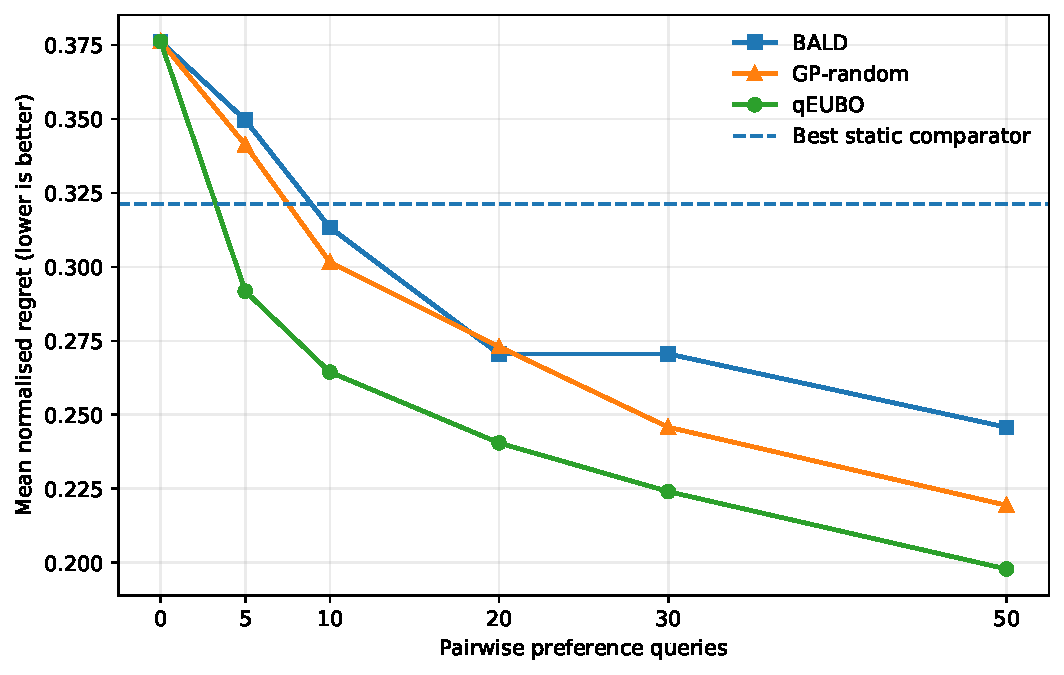
\includegraphics[width=0.92\linewidth]{fig1_learning_curves.pdf}
\caption{Mean normalised regret across the nine pre-specified cells as a function of pairwise preference budget. The dashed line is the best static comparator (mean regret 0.3212). All learned policies use the same Laplace GP preference model.}
\label{fig:learning}
\end{figure}

Table~\ref{tab:curve} reports paired differences relative to the best static comparator. At $T=5$, the qEUBO interval is already entirely below zero ($-0.0294$, 95\% CI $[-0.0470,-0.0123]$). The difference increases to $-0.1234$ at $T=50$.

\begin{table}[t]
\centering
\caption{Paired listener-level differences in normalised regret relative to the best static comparator. Negative values favour the learned method.}
\label{tab:curve}
\begin{tabular}{rrrrrrr}
\toprule
 & \multicolumn{6}{c}{Query budget} \\
\cmidrule(lr){2-7}
Method & 0 & 5 & 10 & 20 & 30 & 50 \\
\midrule
qEUBO & +0.0551 & -0.0294 & -0.0568 & -0.0807 & -0.0972 & -0.1234 \\
BALD & +0.0551 & +0.0285 & -0.0079 & -0.0506 & -0.0506 & -0.0754 \\
GP-random & +0.0551 & +0.0201 & -0.0196 & -0.0482 & -0.0754 & -0.1018 \\
\bottomrule
\end{tabular}
\end{table}

\subsection{Acquisition efficiency}

The matched qEUBO-versus-GP-random comparison isolates active query selection from GP fitting. At five queries, qEUBO reduced regret by $0.0495$ relative to GP-random (95\% CI $[-0.0627,-0.0364]$). At ten queries, the difference was $-0.0371$ (95\% CI $[-0.0489,-0.0252]$). Thus the qEUBO advantage is clearest when the preference budget is small.

At larger budgets the GP-random policy partially catches up. At $T=50$, mean regrets are 0.1978 for qEUBO and 0.2194 for GP-random. This is consistent with qEUBO primarily improving \emph{query allocation efficiency}: with sufficient random comparisons, the shared GP model can eventually identify useful regions, whereas qEUBO reaches lower regret earlier.

\subsection{Context heterogeneity}

The primary $T=20$ effect varies by context (Fig.~\ref{fig:contexts}). Noisy conversation shows a mean difference of $-0.1102$ (95\% CI $[-0.1331,-0.0873]$) and lecture $-0.1124$ (95\% CI $[-0.1415,-0.0835]$). Music is weaker at $-0.0197$ with CI $[-0.0443,+0.0047]$, which includes zero.

\begin{figure}[t]
\centering
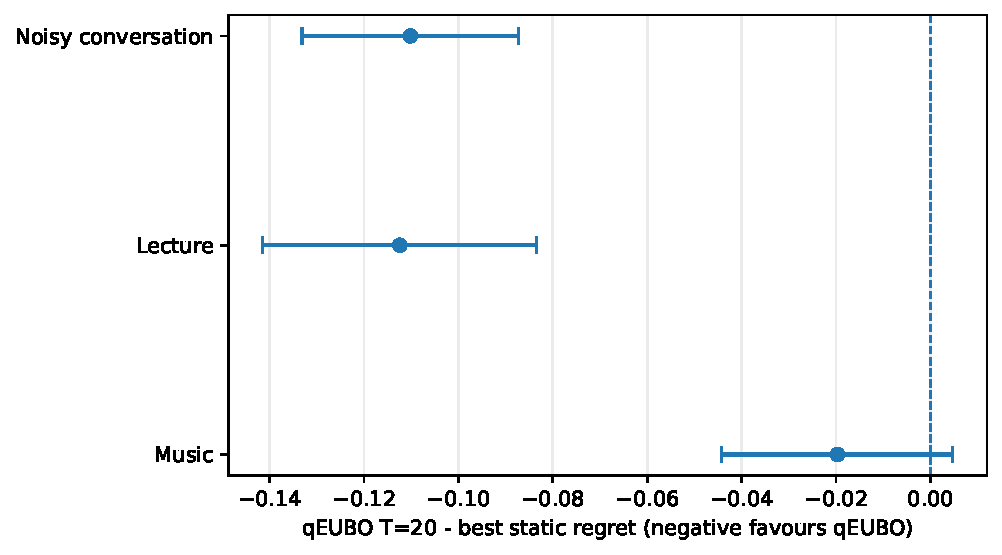
\includegraphics[width=0.88\linewidth]{fig2_context_effects.pdf}
\caption{Context-specific qEUBO $T=20$ paired regret difference relative to the per-cell best static comparator. Error bars are 95\% listener-level bootstrap intervals. Negative values favour qEUBO.}
\label{fig:contexts}
\end{figure}

\subsection{Preference-family heterogeneity}

Effects also vary by preference objective (Fig.~\ref{fig:families}). Comfort shows the largest improvement: $-0.1848$ (95\% CI $[-0.2171,-0.1533]$). The balanced family improves by $-0.0458$ (95\% CI $[-0.0745,-0.0176]$). Intelligibility averaged across contexts is $-0.0117$ with CI $[-0.0420,+0.0189]$, providing no clear aggregate advantage at $T=20$.

\begin{figure}[t]
\centering
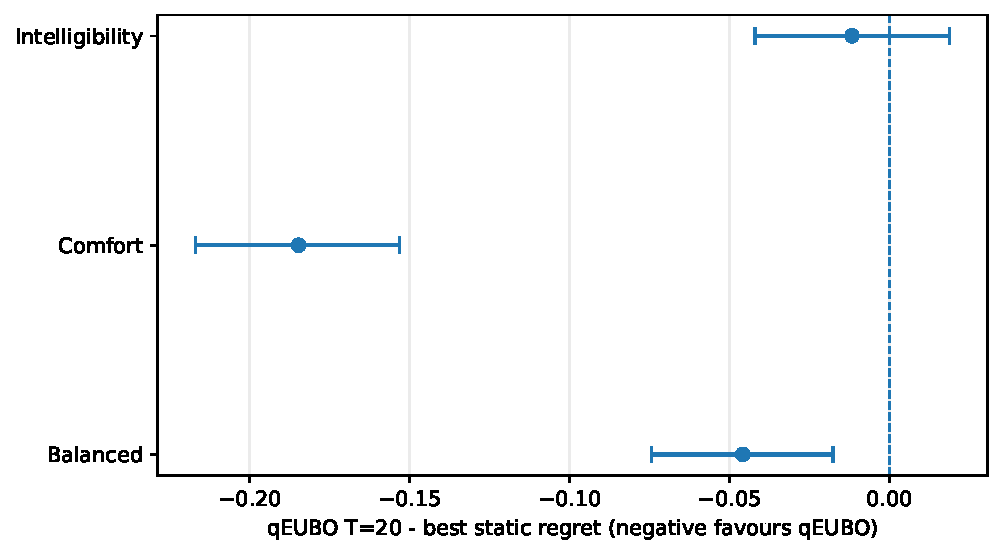
\includegraphics[width=0.88\linewidth]{fig3_family_effects.pdf}
\caption{Preference-family qEUBO $T=20$ paired regret difference relative to best static. Negative values favour qEUBO.}
\label{fig:families}
\end{figure}

\subsection{Context-by-family analysis}

Figure~\ref{fig:heatmap} and Table~\ref{tab:cells} expose the interaction behind the aggregate results. qEUBO improves all three preference families in noisy conversation and lecture. In music, comfort still improves strongly ($-0.1345$), balanced is essentially neutral ($+0.0001$), and intelligibility favours the static comparator ($+0.0754$, 95\% CI $[+0.0371,+0.1132]$).

\begin{figure}[t]
\centering
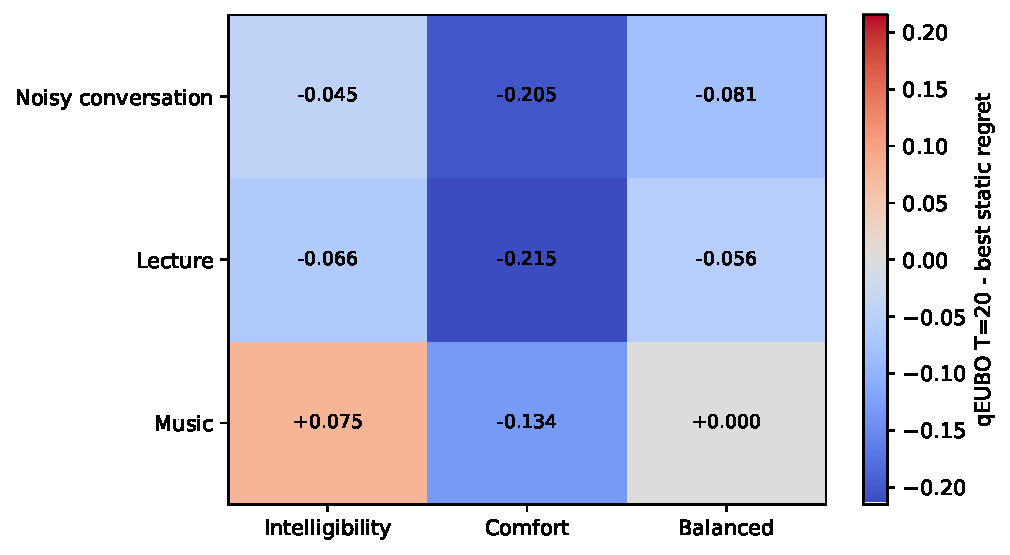
\includegraphics[width=0.88\linewidth]{fig4_context_family_heatmap.pdf}
\caption{Context-by-family mean paired difference for qEUBO at $T=20$ versus best static. Negative values favour qEUBO; positive values favour static fitting.}
\label{fig:heatmap}
\end{figure}

\begin{table}[t]
\centering
\caption{Context-by-family qEUBO $T=20$ differences versus best static.}
\label{tab:cells}
\begin{tabular}{llrr}
\toprule
Context & Family & Mean difference & 95\% CI \\
\midrule
Noisy conversation & Intelligibility & -0.0448 & $[-0.0833,-0.0063]$ \\
Noisy conversation & Comfort & -0.2046 & $[-0.2386,-0.1706]$ \\
Noisy conversation & Balanced & -0.0811 & $[-0.1166,-0.0461]$ \\
Lecture & Intelligibility & -0.0656 & $[-0.1051,-0.0260]$ \\
Lecture & Comfort & -0.2152 & $[-0.2607,-0.1709]$ \\
Lecture & Balanced & -0.0564 & $[-0.0963,-0.0164]$ \\
Music & Intelligibility & +0.0754 & $[+0.0371,+0.1132]$ \\
Music & Comfort & -0.1345 & $[-0.1646,-0.1048]$ \\
Music & Balanced & +0.0001 & $[-0.0358,+0.0368]$ \\
\bottomrule
\end{tabular}
\end{table}

\subsection{Post-hoc noise-sensitive robustness family}

The noise-sensitive family was introduced after a development diagnostic and cannot support the primary claim. It is nevertheless informative as a harder robustness case. qEUBO remains worse than static at $T=5$ ($+0.0633$, 95\% CI $[+0.0339,+0.0922]$) and $T=10$ ($+0.0300$, CI $[+0.0000,+0.0590]$), is indistinguishable at $T=20$ and $T=30$, and becomes clearly better only at $T=50$ ($-0.0446$, CI $[-0.0738,-0.0158]$). This contrasts with the pre-specified population, where qEUBO is already superior by five queries.

\subsection{Post-final development diagnostics conducted after the final evaluation}
\label{sec:reviewdiag}

After completion and analysis of the frozen final cohort, reviewer comments motivated several additional diagnostics. To preserve separation from the final evidence, these analyses were specified in a protocol-v2 addendum before execution, used development seed 424242 only, and did not rerun or modify the reserved final seed. They are therefore exploratory development evidence rather than part of the primary final evaluation.

First, a simple interactive coordinate-search baseline was evaluated on the same 32-listener development sweep used before the final run. At 20 pairwise queries, its listener-mean regret difference relative to the static reference was $+0.0275$ (worse than static), and it beat static for 11/32 listeners. On those same development listeners qEUBO was $-0.0566$ relative to static and beat static for 21/32 listeners. Thus a simple local interactive strategy did not reproduce the gain of the GP-based active policy under the tested budget.

Second, we examined query geometry to understand the relatively flat BALD trajectory. A query endpoint was labelled ``near boundary'' when $\max_j |z_j|\geq0.9$. Across 32 development listeners, nine primary context/family cells and the first 30 queries, 87.6\% of BALD endpoints were near the boundary compared with 22.9\% for qEUBO. This concentration offers a plausible geometric explanation for BALD spending many mid-budget queries on extreme settings, although the diagnostic is post-final and does not establish causality.

Third, the music--intelligibility failure was probed directly. For all 32 development listeners the approximate oracle optimum placed both noise reduction and speech enhancement essentially at the off corner (mean $z_4=-0.995$, mean $z_5=-0.994$). This confirms an extreme optimum geometry. However, removing the centre-pulling GP mean by setting $\gamma=0$ did \emph{not} improve qEUBO: mean T=20 regret increased from 0.2940 to 0.3815. By contrast, eliminating simulated choice noise and lapses reduced mean T=20 regret to 0.0693 and improved 31/32 listeners. Thus this diagnostic supports the corner observation but not the hypothesis that the quadratic prior is the principal cause; within this development test, response noise was materially involved.

The scripts and outputs for these diagnostics are released under \texttt{publication/reviewer\_diagnostics/}. They are not used to alter the frozen final estimand or confidence interval.


Finally, a small development-only robustness sweep (12 listeners) perturbed assumptions that could favour the learner. The qEUBO T=20 minus static mean remained negative when the listener ideal-gain offset was doubled ($-0.0594$) and under doubled audiogram-observation error ($-0.0481$ among 11 feasible of 12 attempted listeners). Removing the ideal-gain-distance term entirely increased the mean advantage to $-0.1771$. In contrast, doubling simulated choice noise and lapse changed the mean difference to $+0.0482$, favouring static fitting. The high-audiogram-error condition also produced one listener with no feasible low-gain anchor; this draw was recorded as infeasible rather than repaired by relaxing constraints. These small-sample diagnostics indicate that the reported qualitative advantage is not dependent on the ideal-gain term, but is sensitive to preference-response reliability.

\section{Discussion}
\label{sec:discussion}

\subsection{Main finding: decision-theoretic acquisition improves low-budget personalisation}

The principal result is not simply that a GP can learn a simulated listener preference. Prior hearing-aid work already demonstrates that pairwise comparisons and Bayesian models can support personalisation \cite{birlutiu2010,vyas2022,ni2024,ignatenko2025}. The stronger result is that, under matched modelling conditions, \emph{which comparisons are requested} materially changes the recommendation quality at small budgets.

At five queries, qEUBO is already better than the strengthened static reference, while BALD and GP-random remain worse than static on average. qEUBO also beats GP-random directly by nearly 0.05 normalised-regret units. At ten queries the qEUBO-versus-random advantage remains substantial. The convergence of policies at larger budgets further supports an efficiency interpretation: random exploration eventually supplies the GP with useful coverage, but qEUBO places early queries in regions that more directly improve the terminal recommendation.

A post-final development diagnostic also clarifies BALD's weak mid-budget behaviour: 87.6\% of BALD query endpoints lay near the latent boundary ($\max|z|\geq0.9$), compared with 22.9\% for qEUBO. This suggests that the information-gain objective devoted substantially more comparisons to extreme settings, whereas qEUBO concentrated more of its budget away from the boundary. Because this analysis was requested after the final study, it is presented as explanatory evidence rather than a pre-specified result.

This distinction matters in human-in-the-loop applications. A comparison is not free: it consumes attention, can induce fatigue and may become less reliable with repeated exposure. The practical target is therefore not merely asymptotic preference-function recovery; it is acceptable decision quality after a small number of interactions. qEUBO's decision-theoretic objective is aligned with that target.

\subsection{Strength of the static comparator}

The primary analysis takes the per-cell minimum across three recorded static rows, but the correction above is important for interpretation: only two distinct primary utility behaviours are represented. The default and slow rows have identical utility because compression speed is absent from the three pre-specified primary families. The linear row is more than a compression-only alternative: it also switches noise reduction and speech enhancement off. Consequently, the reported static reference should be understood as the better of two distinct synthetic static behaviours, not as three independent prescriptions.

This reference remains stronger than comparing only with the default half-gain setting because each cell may retrospectively choose between the default behaviour and the linear/NR-off/SE-off behaviour. However, the earlier manuscript description as a ``best of three'' distinct alternatives overstated baseline diversity; the revised wording and released rows make the exact comparison explicit.

\subsection{Why comfort is easier to improve than intelligibility}

The large comfort effect and smaller intelligibility effect are plausible given the problem construction and application domain. A prescription rule is already designed to supply audibility and speech-oriented gain from audiometric information. The room for preference optimisation may therefore be smaller when the hidden objective is dominated by an intelligibility-like term.

Comfort is more idiosyncratic. Listener-specific upper limits, preferred gain offsets and processing penalties create heterogeneous optima that cannot be recovered from the audiogram alone. Pairwise preference learning has more information to add in this setting. This pattern is consistent with self-fitting studies showing that user-selected settings often remain near prescription-derived solutions while exhibiting systematic individual deviations \cite{dreschler2008,sabin2020}.

\subsection{Context matters}

Noisy conversation and lecture exhibit robust qEUBO gains, whereas music is weak overall. The context-by-family analysis makes the reason visible: music-comfort benefits strongly, but music-intelligibility is a clear negative result.

This failure case should not be treated as noise to be averaged away. The post-final development diagnostic in Section~\ref{sec:reviewdiag} shows that the music--intelligibility optimum is consistently located at an extreme NR/SE-off corner. That geometry is therefore real in the simulator. The diagnostic did not support a simple ``prior pulls away from the corner'' explanation: setting the quadratic-prior coefficient to zero worsened performance. Conversely, removing simulated response noise/lapses substantially reduced regret, indicating that noisy pairwise decisions interact strongly with the extreme optimum in this condition.

The result also highlights application-model mismatch: the intelligibility-like oracle is speech-oriented, whereas the context is music, and the six latent controls were designed around hearing-aid speech-processing dimensions. A future system should consider context-conditioned models or multi-task kernels rather than assuming uniform preference geometry across contexts. The earlier multi-task preference-learning literature provides a natural starting point \cite{birlutiu2010}.

\subsection{Relation to recent hearing-aid ML}

The present results should be interpreted in the context of increasingly active machine-learning research on hearing-aid personalisation. Nielsen et al. \cite{nielsen2015} already demonstrated GP active learning from pairwise perceptual comparisons in hearing-aid parameter adjustment, while Korzepa et al. \cite{korzepa2020} developed a simulation environment for contextual hearing-aid personalisation. Vyas et al. \cite{vyas2022} demonstrated efficient pairwise identification over a discrete preset set; Ni et al. \cite{ni2024} improved training efficiency through multi-band Bayesian learning and included a small clinical validation; Ignatenko et al. \cite{ignatenko2025} analysed sequential BO with pairwise comparison using hearing-aid fitting as a motivating application.

AudioTwin differs most clearly in experimental emphasis. It treats the final evaluation as a controlled acquisition-policy comparison with a frozen protocol, continuous multidimensional latent control, explicit feasibility projection and an oracle-strengthened static baseline. This allows the study to answer a machine-learning question---whether qEUBO improves recommendation regret under limited preference budgets---without claiming that the simulated utility constitutes clinical evidence.

\subsection{Feasibility constraints and the rejected listener}

The final evaluation includes a useful edge case. One simulated listener admitted no feasible low-gain anchor under the frozen constraints. Rather than weakening constraints after observing the failure, the task was recorded as infeasible and replaced using a deterministic rule defined before performance analysis.

This behaviour is desirable for safety-sensitive optimisation. An algorithm should be allowed to fail closed when the assumed feasible domain is empty. In a real hearing-care workflow, the corresponding response would not be automatic relaxation of model limits; it would be fallback to a verified configuration, additional measurement or professional review.

Again, these constraints are computational guardrails and should not be equated with regulatory or clinical safety guarantees.

\subsection{Protocol discipline as part of applied ML evaluation}

Applied optimisation studies are vulnerable to researcher degrees of freedom. Candidate spaces, baselines, oracle definitions, budgets and random seeds can all be changed after preliminary results are seen. Such adaptation may be necessary during development, but it weakens confirmatory interpretation if the same outcomes are repeatedly reused.

The AudioTwin workflow records development/final separation in its private protocol record. A reserved final seed was not used during method development. The primary endpoint, sample size and bootstrap procedure were specified before final outcome inspection. A development-discovered compression artefact was not inserted into the three pre-specified utility families; instead it was isolated into a post-hoc robustness family. The original development branch and annotated tags are now public, but they remain repository provenance rather than an externally registered protocol. These choices do not eliminate all design bias---the simulator itself was developed by the research team---but they reduce direct tuning to the reported final random draw.

\section{Limitations}
\label{sec:limitations}

\subsection{Simulation is not clinical validation}

The most important limitation is that all 128 final listeners are simulated. The oracle contains plausible ingredients---audibility, comfort, ideal-gain deviation, compression preference and response noise---but it is not a human participant. Lower oracle regret demonstrates successful optimisation of the specified benchmark, not improved hearing outcomes.

This limitation is particularly important because recent hearing-aid personalisation studies include real participant data \cite{vyas2022,ni2024}. AudioTwin should therefore be viewed as a methodological and reproducibility study that motivates, rather than replaces, a human-listener trial.

\subsection{The oracle and learner share structural assumptions}

Although the oracle is not directly exposed to the learner, both are smooth functions over the same latent DSP space, and the oracle's hidden ideal gain is derived from the same half-gain prescription family used by the learner, plus random listener-specific offsets. These shared structural assumptions make the benchmark favourable to smooth preference learning and limit external validity. Real preferences may include discontinuities, hysteresis, context drift, adaptation and non-stationary judgement noise. Post-final development-only robustness experiments are therefore governed by the post-final protocol-v2 addendum; they cannot alter the frozen final primary result.

\subsection{Approximate optimum and normalised regret}

The oracle optimum is computed numerically rather than analytically, using a random-plus-evolutionary search specified in the frozen experiment. Regret is therefore measured relative to an approximate feasible optimum. This is suitable for comparing methods under the same benchmark but introduces numerical approximation error into the absolute regret scale.

\subsection{Known rather than learned constraints}

AudioTwin projects candidates against known model constraints. It does not infer safety from observations and therefore does not solve the full safe-BO problem addressed by methods such as SafeOpt \cite{sui2015}. Applications with uncertain constraints would require a probabilistic constraint model and a different safety analysis.

\subsection{Limited DSP and context model}

The six-dimensional latent space omits many commercial hearing-aid features, including binaural coordination, adaptive directionality, feedback cancellation, source separation and modern neural speech enhancement. The three final contexts likewise cover only a small subset of real environments. The reported effects should not be extrapolated to a complete hearing-aid signal chain.

\subsection{No computational-time or human-fatigue outcome}

The study counts preference comparisons but does not model response time, fatigue or cognitive burden. Pairwise queries with similar candidates may be information-rich yet perceptually difficult. Human studies should jointly optimise statistical efficiency and usability.

\section{Future work}
\label{sec:future}

The highest-priority next step is a prospective listening study. A suitable initial design would compare a verified prescription, conventional fine-tuning and AudioTwin-qEUBO within participants. Outcomes should include preference, speech recognition in noise, comfort, listening effort, test--retest stability and the number of comparisons required to reach a stable setting. Stimulus duration should be chosen with reference to evidence that preference reliability depends on the amount of speech presented \cite{whitmer2022}.

A second direction is hierarchical preference learning. Existing work suggests that preference structure can be shared across listeners \cite{birlutiu2010}; a population prior could reduce cold-start queries while retaining individual adaptation.

A third direction is explicit context transfer. Instead of fitting each context independently, a multi-task kernel could share statistical strength between noisy conversation and lecture while allowing music to retain a distinct latent function. The negative music-intelligibility result makes this a particularly testable hypothesis.

Finally, learned constraints and modern neural audio processing could be integrated. The optimisation layer could tune parameters of speech enhancement or source-separation systems, while a probabilistic safety/quality model excludes settings with unacceptable distortion. Such extensions would move AudioTwin from a controlled DSP testbed towards a broader human-centred machine-learning framework.

\section{Conclusion}
\label{sec:conclusion}

AudioTwin formulates personalised hearing-aid fitting as constrained preferential Bayesian optimisation. In a frozen final evaluation of 128 simulated listeners, qEUBO reduced mean normalised regret from 0.3212 for an oracle-strengthened static comparator to 0.2405 after 20 pairwise choices, a 25.1\% reduction. The primary paired difference was $-0.0807$ with 95\% listener-level bootstrap CI $[-0.1027,-0.0593]$.

More importantly for the machine-learning contribution, qEUBO outperformed a matched GP-random acquisition policy at five and ten comparisons. This demonstrates an early-budget benefit attributable to active query selection rather than GP preference modelling alone. Performance was heterogeneous: comfort-oriented and speech-oriented contexts showed the largest gains, whereas music-intelligibility favoured static fitting at the primary budget.

These results support qEUBO as a promising acquisition strategy for sparse, noisy personalisation problems with known feasibility constraints. They do not establish clinical benefit. The next evidential step is human-listener validation under realistic speech and acoustic conditions.

\section*{CRediT authorship contribution statement}
Alan Immanuel Benjamin Vallavaraj: Conceptualisation, Methodology, Software, Validation, Formal analysis, Investigation, Data curation, Visualisation, Writing -- original draft, Writing -- review \& editing, Project administration.

\section*{Funding}
This research did not receive any specific grant from funding agencies in the public, commercial, or not-for-profit sectors.

\section*{Declaration of competing interest}
The author declares no known competing financial interests or personal relationships that could have appeared to influence the work reported in this paper.

\section*{Ethics statement}
The reported final evaluation is a computational simulation and did not recruit human participants or use identifiable participant data. Human-participant ethics approval was therefore not required for the experiments reported here. Any prospective human-listener validation will require appropriate institutional ethics review and informed consent.

\section*{Data and code availability}
The AudioTwin source code, protocol record, exact analysis implementation, LaTeX manuscript sources and consolidated final synthetic dataset are available at \url{https://github.com/alanvallavaraj/AudioTwin}. The released file \texttt{publication/data/final\_v1.parquet} contains all 32,256 final analysis rows and is accepted directly by \texttt{scripts/analyze\_final.py}; it is sufficient to recompute the reported listener-level bootstrap confidence intervals. Exact package versions from the QMUL final-run environment are pinned in \texttt{requirements-final.txt}. The repository is released under the MIT License. The curated \texttt{main} history is post-experiment; the original development lineage and annotated protocol tags are published separately under \texttt{protocol-history} and documented in \texttt{PROTOCOL\_PROVENANCE.md}.

\section*{Declaration of generative AI and AI-assisted technologies in the manuscript preparation process}
During the preparation of this work, the author used ChatGPT (OpenAI) to assist with manuscript organisation, language refinement, LaTeX preparation and consistency checking. The author reviewed and edited the generated material, verified the reported numerical results against the frozen analysis outputs, and takes full responsibility for the content of the publication.

\section*{Acknowledgements}
The author acknowledges computational resources used for the final simulation experiments and institutional research support from the University of Westminster. No human participant contributed data to the reported final evaluation.

\bibliographystyle{elsarticle-num}
\bibliography{references}

\end{document}
